\documentclass{article}
\usepackage[utf8]{inputenc}
\usepackage[spanish]{babel}
\usepackage{graphicx}
\usepackage{longtable}
\graphicspath{{./img/}}

\title{Práctica 1. Análisis de eficiencia de algoritmos}
\author{Noelia Escalera Mejías \\
		\and Alejandro Menor Molinero \\
		\and Javier Núñez Suárez \\
		\and Adra Sánchez Ruiz \\
		\and Jesús Torres Sánchez}
	
\begin{document}
	\maketitle
	\section{Introducción}
	\section{Eficiencia empírica}
	\subsection{Algoritmos de ordenación rápidos}
		\begin{longtable}{|c|c|c|c|}
			\hline
			Tamaño del vector & Tiempo con Quicksort & Tiempo con Mergesort & Tiempo con Heapsort \\ \hline
			500	     &  0.000125572	 &  0.000185121	 &  0.000192113  \\ \hline
			1000	 &  0.000271314	 &  0.000389135	 &  0.000444516  \\ \hline
			1500	 &  0.00041891	 &  0.000760708	 &  0.000705254  \\ \hline
			2000	 &  0.000594146	 &  0.00102568	 &  0.00097424  \\ \hline
			2500	 &  0.000740502	 &  0.000482617	 &  0.000443686  \\ \hline
			3000	 &  0.000596825	 &  0.000494674	 &  0.000381796  \\ \hline
			3500	 &  0.000343663	 &  0.000452999	 &  0.000429375  \\ \hline
			4000	 &  0.000373585	 &  0.000644118	 &  0.00053697  \\ \hline
			4500	 &  0.00042863	 &  0.000694048	 &  0.000605903  \\ \hline
			5000	 &  0.000513286	 &  0.000788472	 &  0.000634107  \\ \hline
			5500	 &  0.000557894	 &  0.000948842	 &  0.000715611  \\ \hline
			6000	 &  0.000605284	 &  0.00105457	 &  0.000794382  \\ \hline
			6500	 &  0.000657624	 &  0.000926247	 &  0.000862167  \\ \hline
			7000	 &  0.000714435	 &  0.00100227	 &  0.000929307  \\ \hline
			7500	 &  0.000757684	 &  0.0011178	 &  0.00100083  \\ \hline
			8000	 &  0.000831217	 &  0.00123515	 &  0.00108477  \\ \hline
			8500	 &  0.00087632	 &  0.00131409	 &  0.00114999  \\ \hline
			9000	 &  0.000951436	 &  0.00139895	 &  0.00124178  \\ \hline
			9500	 &  0.00100672	 &  0.00153253	 &  0.001302  \\ \hline
			10000	 &  0.00104054	 &  0.00163203	 &  0.00136841  \\ \hline
			10500	 &  0.00111741	 &  0.00176789	 &  0.00144557  \\ \hline
			11000	 &  0.0011769	 &  0.00188453	 &  0.00152554  \\ \hline
			11500	 &  0.00124374	 &  0.00208893	 &  0.00161126  \\ \hline
			12000	 &  0.00128353	 &  0.00217296	 &  0.00168296  \\ \hline
			12500	 &  0.00134991	 &  0.00229752	 &  0.0017724  \\ \hline
			13000	 &  0.00142095	 &  0.00192418	 &  0.00186281  \\ \hline
			13500	 &  0.00144951	 &  0.00202339	 &  0.00193143  \\ \hline
			14000	 &  0.00152673	 &  0.00208988	 &  0.00199139  \\ \hline
			14500	 &  0.00158276	 &  0.00219523	 &  0.00207509  \\ \hline
			15000	 &  0.0016307	 &  0.00232089	 &  0.00216104  \\ \hline
			15500	 &  0.0016855	 &  0.0024091	 &  0.00223611  \\ \hline
			16000	 &  0.00175315	 &  0.00251567	 &  0.00231843  \\ \hline
			16500	 &  0.00180967	 &  0.00262037	 &  0.00240901  \\ \hline
			17000	 &  0.00187919	 &  0.0027362	 &  0.00250793  \\ \hline
			17500	 &  0.00192917	 &  0.00287752	 &  0.00256264  \\ \hline
			18000	 &  0.0020248	 &  0.00300007	 &  0.00263882  \\ \hline
			18500	 &  0.00204495	 &  0.00310153	 &  0.00272534  \\ \hline
			19000	 &  0.00211357	 &  0.00325465	 &  0.00280503  \\ \hline
			19500	 &  0.00218022	 &  0.00338002	 &  0.00289392  \\ \hline
			20000	 &  0.00223461	 &  0.00350399	 &  0.00304415  \\ \hline
			20500	 &  0.00232654	 &  0.00358945	 &  0.00314781  \\ \hline
			21000	 &  0.0023512	 &  0.00372468	 &  0.00322618  \\ \hline
			21500	 &  0.0024141	 &  0.00385273	 &  0.00330935  \\ \hline
			22000	 &  0.00248485	 &  0.00398946	 &  0.00339943  \\ \hline
			22500	 &  0.00255673	 &  0.00411845	 &  0.00348261  \\ \hline
			23000	 &  0.00264539	 &  0.00433311	 &  0.00357741  \\ \hline
			23500	 &  0.00272772	 &  0.00445179	 &  0.00366066  \\ \hline
			24000	 &  0.00270691	 &  0.00454967	 &  0.00373309  \\ \hline
			24500	 &  0.00285553	 &  0.00466454	 &  0.00382896  \\ \hline
			25000	 &  0.00282962	 &  0.0048426	 &  0.00392208  \\ \hline
		\end{longtable}
		\begin{center}
		\tiny Tabla comparativa de tiempos
		\end{center}
		\begin{figure}[h]
		\centering
		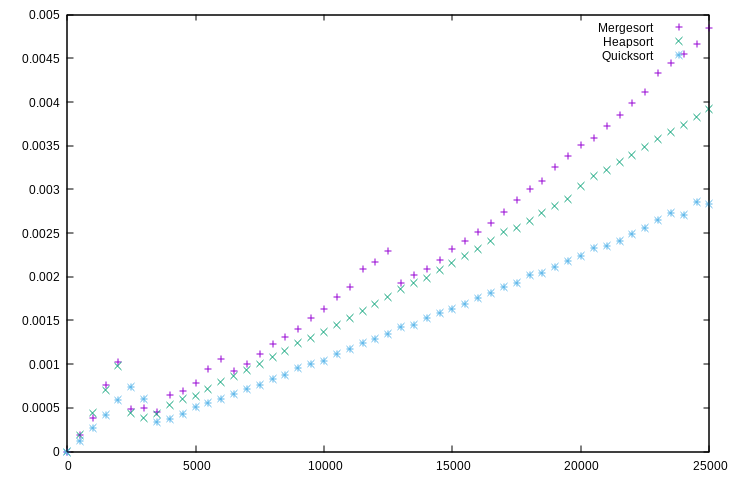
\includegraphics[totalheight=8cm]{img/ordenacion_rapida}
		\caption{Comparación gráfica del rendimiento de los algoritmos de ordenación rápida}
		\label{fig:ordenacion_rapida}
		\end{figure}
		\
	\subsection{Algoritmos de ordenación lentos}
		\begin{longtable}{|c|c|c|c|}
			\hline
			Tamaño del vector & Tiempo con Burbuja & Tiempo con Selección & Tiempo con Inserción \\ \hline
			500	   &    0.00178596	&  0.00147628  	   &  0.00114028   \\ \hline
			1000  &	    0.0028655	&  0.0022588  	   &  0.00172961   \\ \hline
			1500  &	    0.00448784	&  0.00309903  	   &  0.00230721   \\ \hline
			2000  &	    0.00786624	&  0.00525987  	   &  0.00405115   \\ \hline
			2500  &	    0.0124692	&  0.00811555  	   &  0.00630397   \\ \hline
			3000  &	    0.0181514	&  0.0116717  	   &  0.00910679   \\ \hline
			3500  &	    0.0252785	&  0.0157854  	   &  0.0125022   \\ \hline
			4000  &	    0.0337448	&  0.0205625  	   &  0.0158871   \\ \hline
			4500  &	    0.0436306	&  0.0268227  	   &  0.0201791   \\ \hline
			5000  &	    0.0551609	&  0.0331552  	   &  0.026194   \\ \hline
			5500  &	    0.0681233	&  0.0401148  	   &  0.030802   \\ \hline
			6000  &	    0.0824843	&  0.0467118  	   &  0.035932   \\ \hline
			6500  &	    0.0984357	&  0.0540054   	   &  0.042335   \\ \hline
			7000  &	    0.11589	    &  0.0626111   	   &  0.0497211   \\ \hline
			7500  &	    0.135017	&  0.0717969   	   &  0.0573054   \\ \hline
			8000  &	    0.155683	&  0.0817153   	   &  0.0657382   \\ \hline
			8500  &	    0.176902	&  0.0921947   	   &  0.0768291   \\ \hline
			9000  &	    0.199919	&  0.103297	       &  0.0861508   \\ \hline
			9500  &	    0.225075	&  0.115035	       &  0.0981397   \\ \hline
			10000  &	0.251881	&  0.127486	       &  0.103923   \\ \hline
			10500  &	0.279234	&  0.140492	       &  0.122772   \\ \hline
			11000  &	0.309941	&  0.154166	       &  0.131101   \\ \hline
			11500  &	0.34121	    &  0.171219	       &  0.142071   \\ \hline
			12000  &	0.371406	&  0.183355	       &  0.158711   \\ \hline
			12500  &	0.405278	&  0.198969	       &  0.168258   \\ \hline
			13000  &	0.441736	&  0.215243	       &  0.178126   \\ \hline
			13500  &	0.478529	&  0.232051	       &  0.195711   \\ \hline
			14000  &	0.517851	&  0.249406	       &  0.215179   \\ \hline
			14500  &	0.557069	&  0.26754	       &  0.223471   \\ \hline
			15000  &	0.623507	&  0.286271	       &  0.245298   \\ \hline
			15500  &	0.64346	    &  0.305662	       &  0.257939   \\ \hline
			16000  &	0.693738	&  0.325702	       &  0.277471   \\ \hline
			16500  &	0.734539	&  0.346204	       &  0.297803   \\ \hline
			17000  &	0.778796	&  0.367458	       &  0.311583   \\ \hline
			17500  &	0.829418	&  0.39475	       &  0.322414   \\ \hline
			18000  &	0.880487	&  0.412826	       &  0.352076   \\ \hline
			18500  &	0.933294	&  0.435126	       &  0.360694   \\ \hline
			19000  &	0.986121	&  0.460939	       &  0.379935   \\ \hline
			19500  &	1.07066	    &  0.483263	       &  0.396013   \\ \hline
			20000  &	1.09964	    &  0.515923	       &  0.421674   \\ \hline
			20500  &	1.15639	    &  0.544332	       &  0.447574   \\ \hline
			21000  &	1.22045	    &  0.5604	       &  0.471736   \\ \hline
			21500  &	1.32645	    &  0.590167	       &  0.483069   \\ \hline
			22000  &	1.39171	    &  0.618805	       &  0.504104   \\ \hline
			22500  &	1.55601	    &  0.646724	       &  0.53811   \\ \hline
			23000  &	1.52041	    &  0.671924	       &  0.56646   \\ \hline
			23500  &	1.60414	    &  0.701547	       &  0.596336   \\ \hline
			24000  &	1.6872	    &  0.745452	       &  0.613182   \\ \hline
			24500  &	1.7148	    &  0.770377	       &  0.635088   \\ \hline
			25000  &	1.78348	    &  0.79409	       &  0.638414   \\ \hline
		\end{longtable}
	\begin{figure}[h]
		\centering
		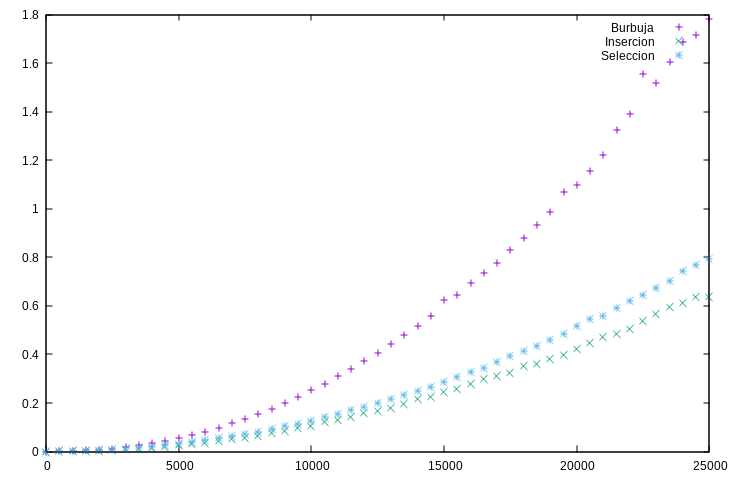
\includegraphics[totalheight=8cm]{img/ordenacion_lenta}
		\caption{Comparación gráfica del rendimiento de los algoritmos de ordenación lenta}
		\label{fig:ordenacion_lenta}
	\end{figure}
	\begin{figure}[h]
		\centering
		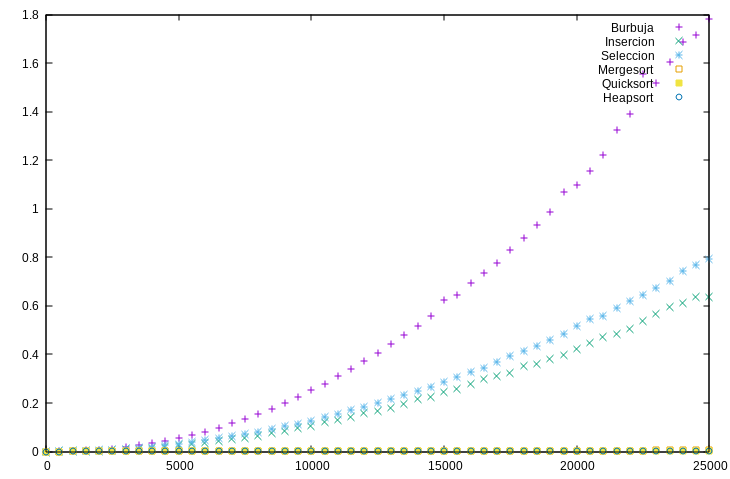
\includegraphics[totalheight=8cm]{img/ordenacion}
		\caption{Comparación gráfica del rendimiento de los algoritmos de ordenación}
		\label{fig:ordenacion}
	\end{figure}
	\begin{figure}[h]
		\centering
		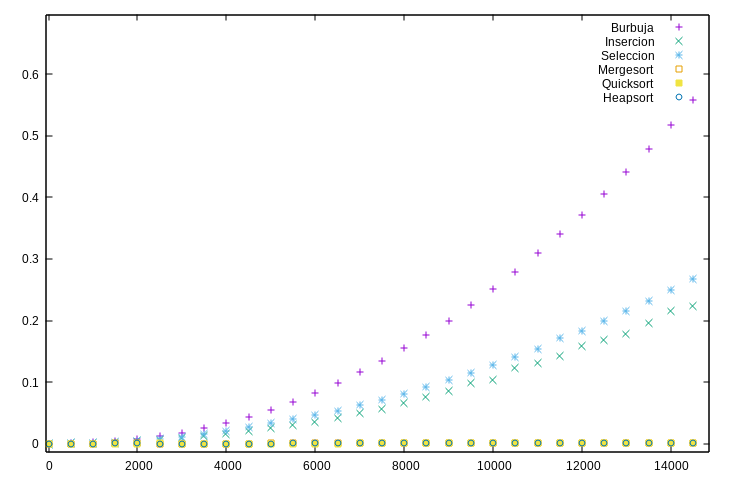
\includegraphics[totalheight=8cm]{img/ordenacion_zoom}
		\caption{Zoom en el intervalo [0-15000] de la figura \ref{fig:ordenacion}}
		\label{fig:ordenacion_zoom}
	\end{figure}

	\section{Eficiencia híbrida}
	Ajuste de las diferentes funciones de acuerdo a la eficiencia teórica de los algoritmos y los datos obtenidos en la eficiencia empírica.
	
	\subsection{Algoritmos de ordenación rápidos}
	
	
	Para el algoritmo Mergesort:

	\begin{longtable}{|c|c|c|}
		\hline
	 	Constante		& Valor			& Error estándar	\\ \hline
		a0              & 3.66473e-12	& 12.16 \\ \hline
		a1              & 8.67345e-08	& 13.28 \\ \hline
		a2              & 0.000308646	& 20.18 \\ \hline
	\end{longtable}

	\begin{figure}[h]
		\centering
		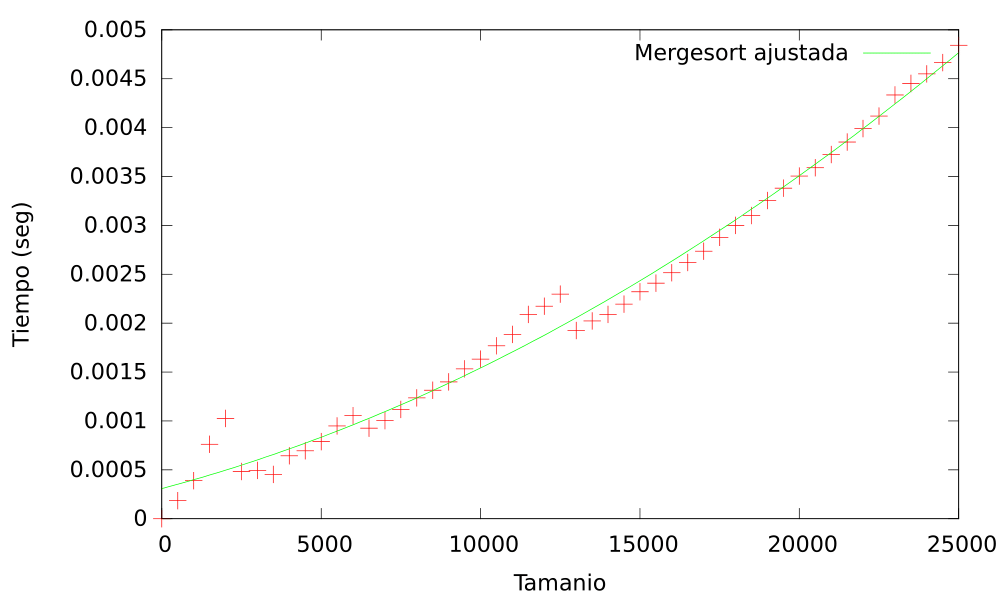
\includegraphics[totalheight=8cm]{img/Mergesort_ajustada}
		\caption{Ajuste función Mergesort}
		\label{fig:Mergesort_ajustada}
	\end{figure}

	Para el algoritmo Heapsort:

	\begin{longtable}{|c|c|c|}
		\hline
		Constante		& Valor			& Error estándar	\\ \hline
		a0              & 2.32227e-12	& 14.09 \\ \hline
		a1              & 9.24005e-08	& 9.152 \\ \hline
		a2              & 0.000224702	& 20.34 \\ \hline
	\end{longtable}

	\begin{figure}[h]
		\centering
		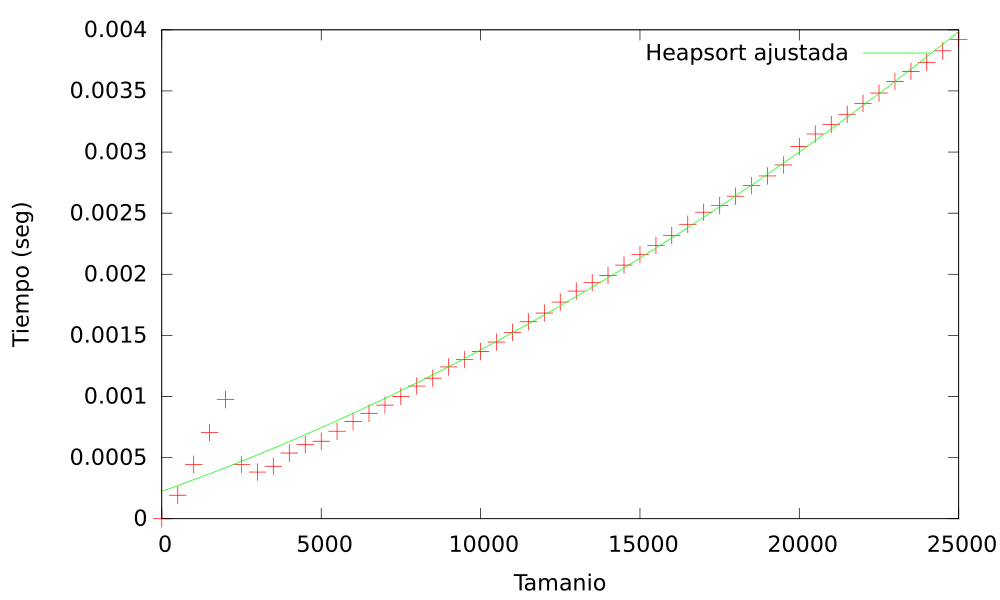
\includegraphics[totalheight=8cm]{img/Heapsort_ajustada}
		\caption{Ajuste función Heapsort}
		\label{fig:Heapsort_ajustada}
	\end{figure}

	Para el algoritmo Quicksort:

	\begin{longtable}{|c|c|c|}
		\hline
		Constante		& Valor			& Error estándar	\\ \hline
		a0              & 1.37793e-12	& 18.84 \\ \hline
		a1              & 7.47827e-08	& 8.974 \\ \hline
		a2              & 0.000181972	& 19.93 \\ \hline
	\end{longtable}
	
	

	\begin{figure}[h]
		\centering
		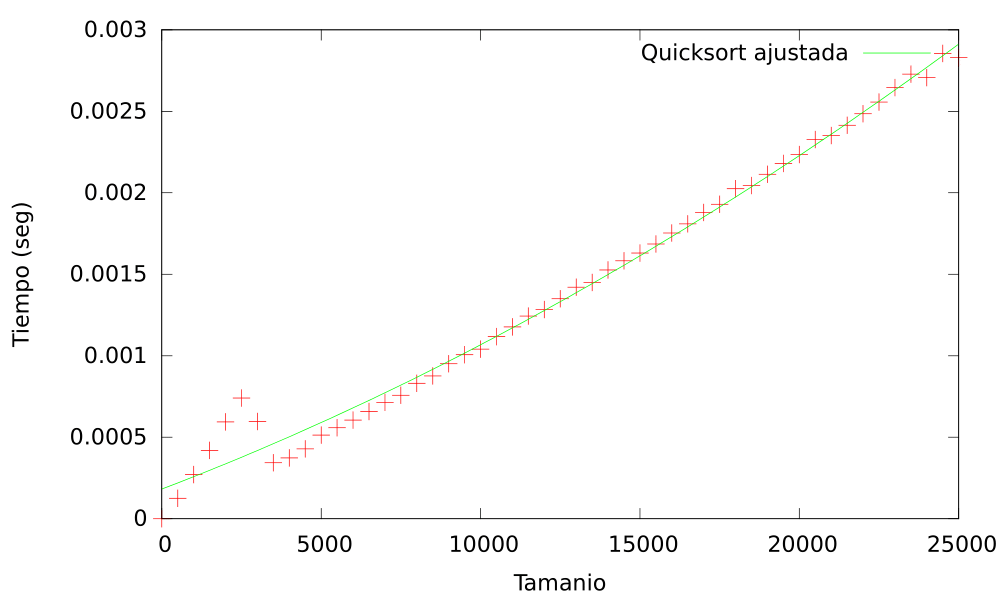
\includegraphics[totalheight=8cm]{img/Quicksort_ajustada}
		\caption{Ajuste función Quicksort}
		\label{fig:Quicksort_ajustada}
	\end{figure}
	
	
	\begin{figure}[h]
		\centering
		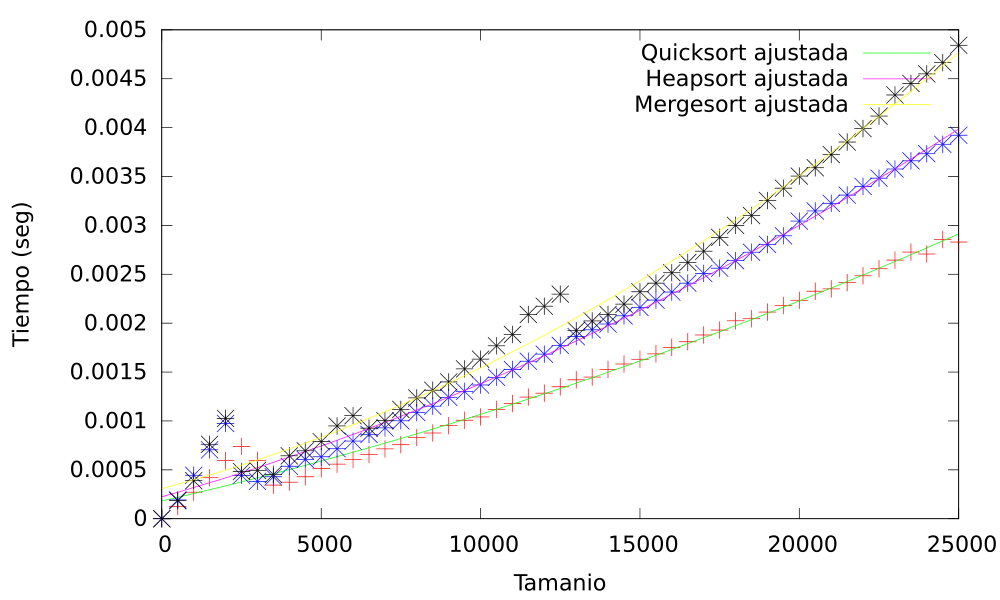
\includegraphics[totalheight=8cm]{img/AlgOrdenacionRapidos_ajustados}
		\caption{Comparativa ajuste para algoritmos de ordenación rápidos}
		\label{fig:AlgOrdenacionRapidos_ajustados}
	\end{figure}

	\subsection{Algoritmos de ordenación lentos}


Para el algoritmo Burbuja:

	\begin{longtable}{|c|c|c|}
		\hline
		Constante		& Valor			& Error estándar	\\ \hline
		a0              & 3.25024e-09	& 1.809 \\ \hline
		a1              & -9.48063e-06	& 16.03 \\ \hline
		a2              & 0.0160101		& 51.32 \\ \hline
	\end{longtable}

	\begin{figure}[h]
		\centering
		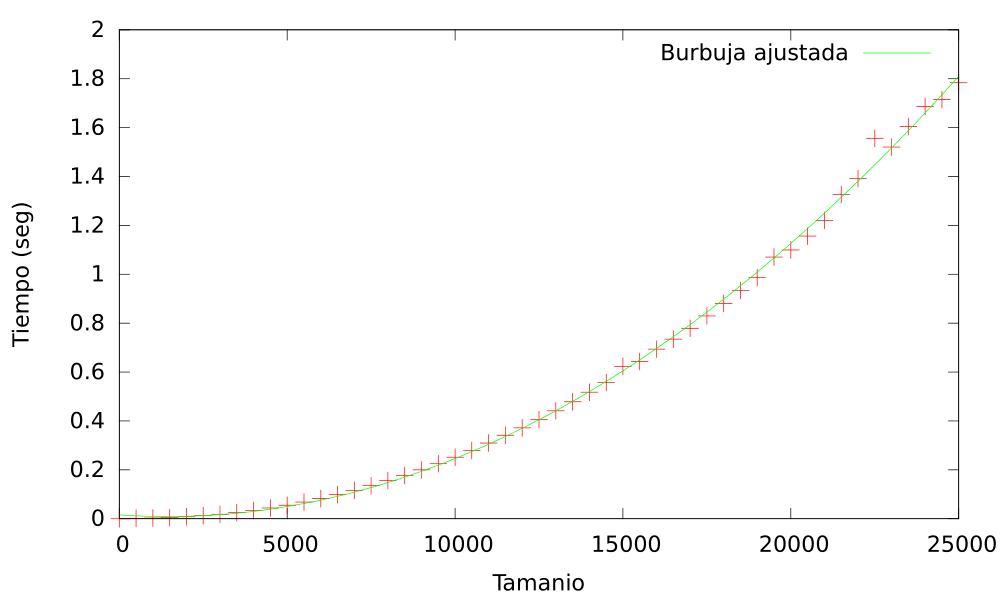
\includegraphics[totalheight=8cm]{img/Burbuja_ajustada}
		\caption{Ajuste función Burbuja}
		\label{fig:Burbuja_ajustada}
	\end{figure}

Para el algoritmo Insercion:

	\begin{longtable}{|c|c|c|}
		\hline
		Constante		& Valor			& Error estándar	\\ \hline
		a0              & 1.02502e-09	& 1.459 \\ \hline
		a1              & 8.53837e-07	& 45.29 \\ \hline
		a2              & -0.00285116	& 73.31 \\ \hline
	\end{longtable}

	\begin{figure}[h]
		\centering
		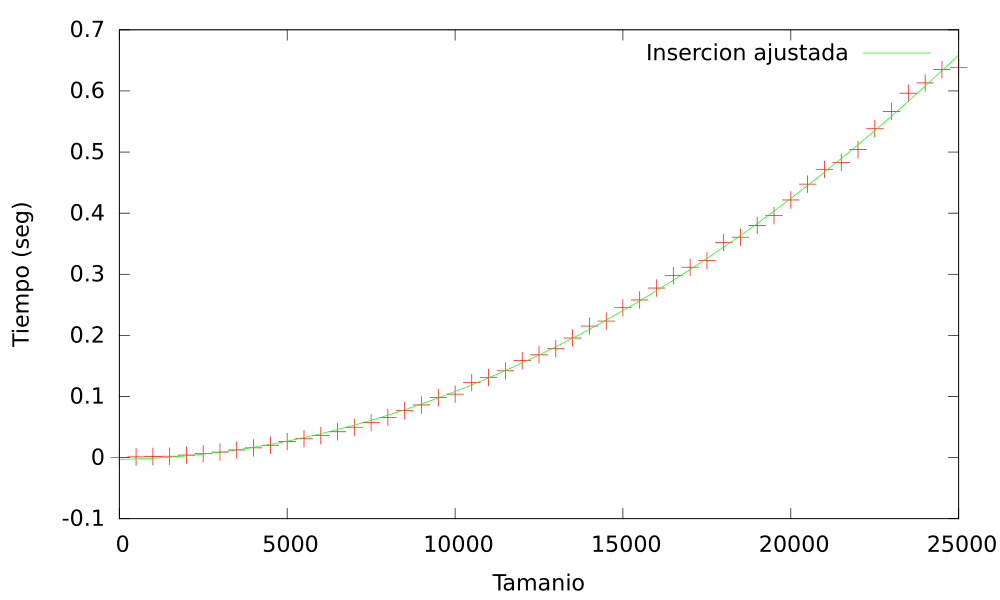
\includegraphics[totalheight=8cm]{img/Insercion_ajustada}
		\caption{Ajuste función Inserción}
		\label{fig:Insercion_ajustada}
	\end{figure}

	Para el algoritmo de Seleccion:

	\begin{longtable}{|c|c|c|}
		\hline
		Constante		& Valor			& Error estándar	\\ \hline
		a0              & 1.28478e-09	& 0.5517 \\ \hline
		a1              & -1.91843e-07	& 95.52 \\ \hline
		a2              & 0.00095162	& 104.1 \\ \hline
	\end{longtable}

	\begin{figure}[h]
		\centering
		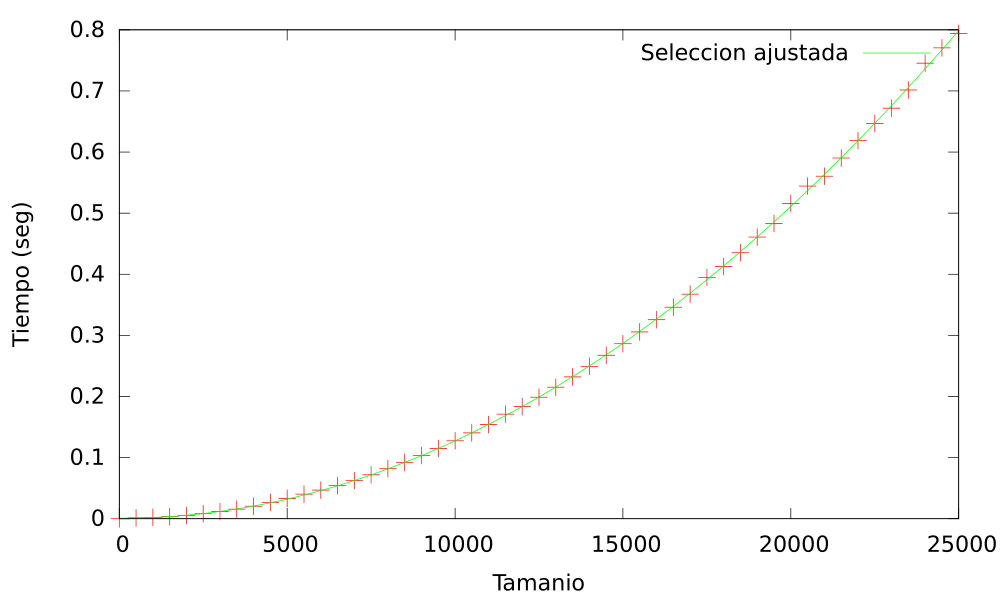
\includegraphics[totalheight=8cm]{img/Seleccion_ajustada}
		\caption{Ajuste función Selección}
		\label{fig:Seleccion_ajustada}
	\end{figure}
	
	\begin{figure}[h]
		\centering
		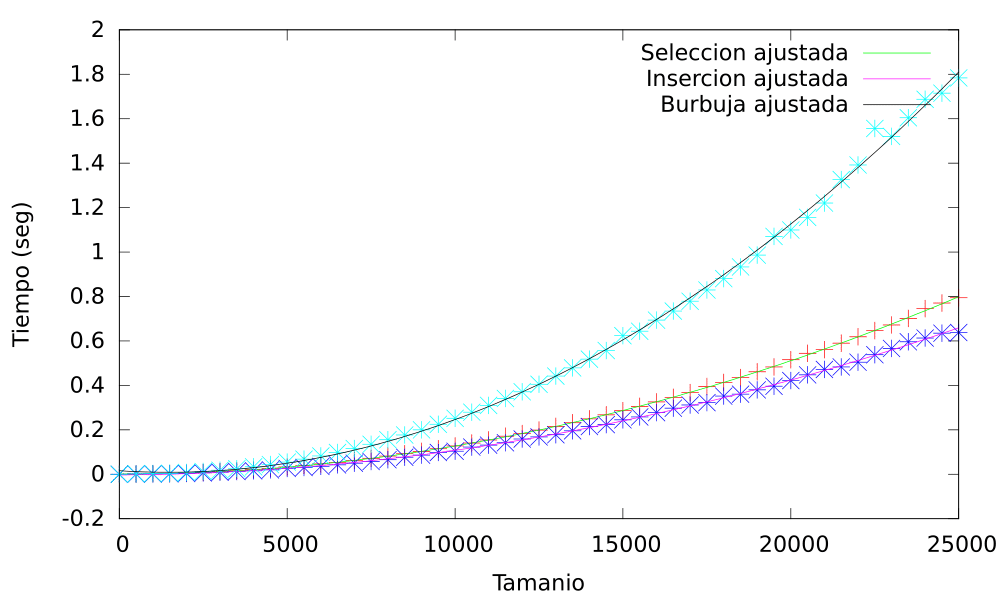
\includegraphics[totalheight=8cm]{img/AlgOrdenacionLentos_ajustados}
		\caption{Comparativa ajuste para algoritmos de ordenación lentos}
		\label{fig:AlgOrdenacionLentos_ajustados}
	\end{figure}
	
	
	\subsection{Algoritmo de Fibonacci}
	
	
	\begin{longtable}{|c|c|c|}
		\hline
		Constante		& Valor			& Error estándar	\\ \hline
		a0              & 2.9613e-09	& 0.2375 \\ \hline
	\end{longtable}

	\begin{figure}[h]
		\centering
		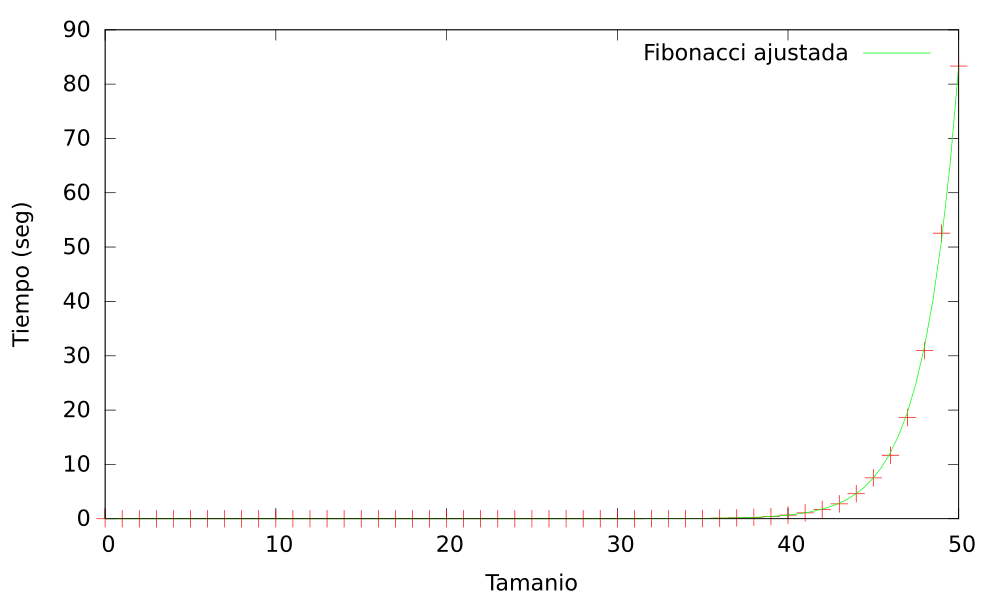
\includegraphics[totalheight=8cm]{img/Fibonacci_ajustada}
		\caption{Ajuste función de Fibonacci}
		\label{fig:Fibonacci_ajustada}
	\end{figure}
	
	\subsection{Algoritmo de Floyd}
	
	
	\begin{longtable}{|c|c|c|}
		\hline
		Constante		& Valor			& Error estándar	\\ \hline
		a0              & 4.5232e-09	& 12.19 \\ \hline
		a1              & 1.64e-06		& 51.27 \\ \hline
		a2              & -0.000541551	& 66.61 \\ \hline
		a3              & 0.0340052		& 121.6 \\ \hline
	\end{longtable}
	
	\begin{figure}[h]
		\centering
		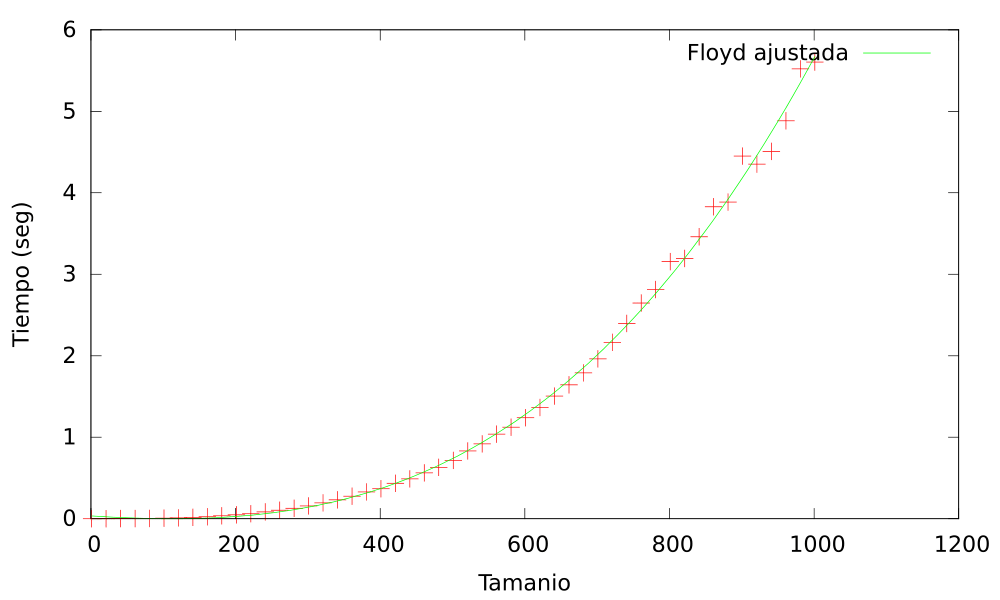
\includegraphics[totalheight=8cm]{img/Floyd_ajustada}
		\caption{Ajuste función de Floyd}
		\label{fig:Floyd_ajustada}
	\end{figure}
	
	\subsection{Ajustes de tiempos con funciones no correspondientes}
	
	\begin{figure}[h]
		\centering
		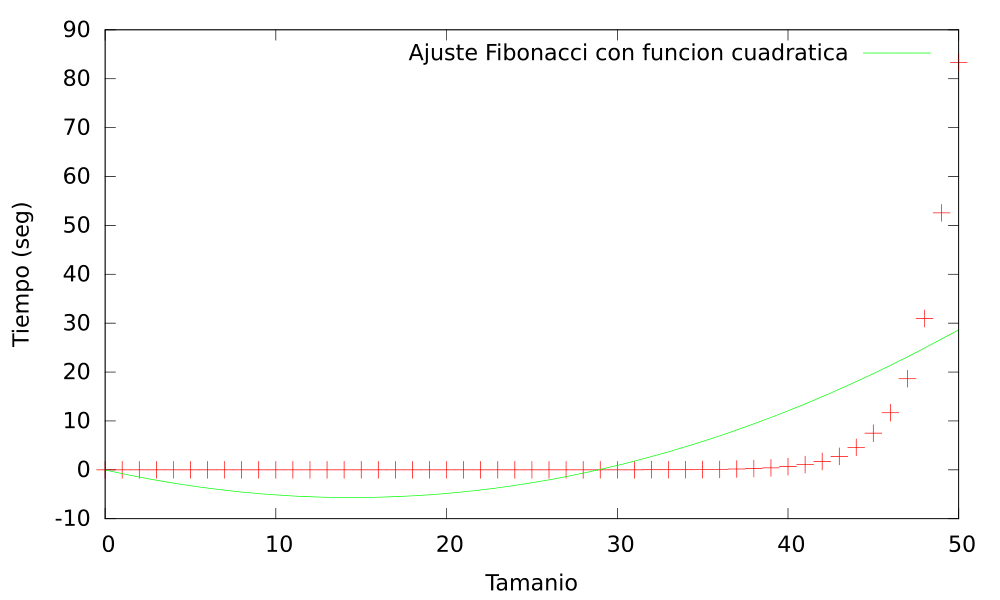
\includegraphics[totalheight=8cm]{img/ajusteFibonacci_cuadratico}
		\caption{Ajuste Fibonacci con función cuadrática}
		\label{fig:ajusteFibonacci_cuadratico}
	\end{figure}
	
	\begin{figure}[h]
		\centering
		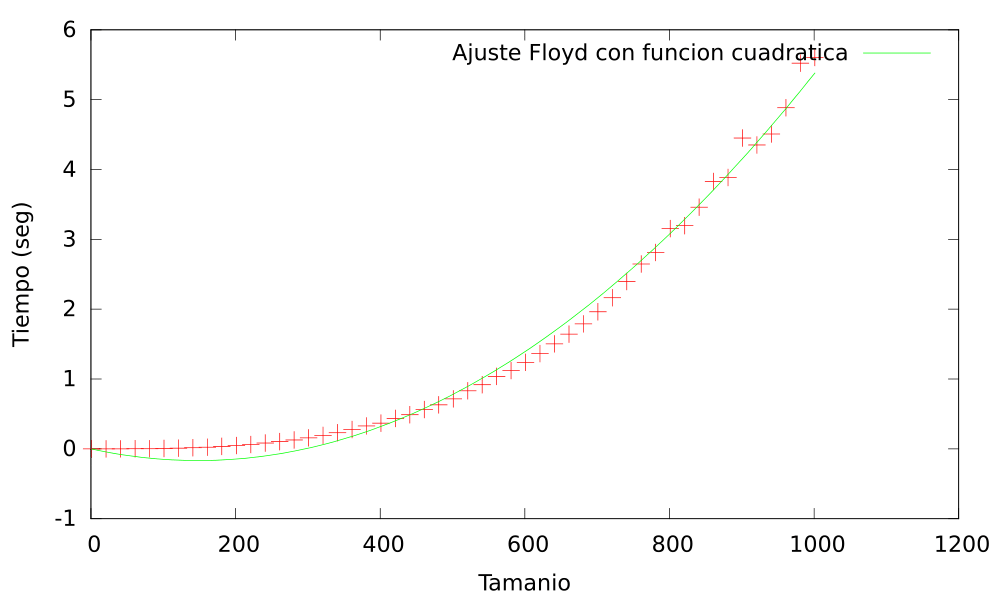
\includegraphics[totalheight=8cm]{img/ajusteFloyd_cuadratico}
		\caption{Ajuste Floyd con función cuadrática}
		\label{fig:ajusteFloyd_cuadratico}
	\end{figure}
	
	\begin{figure}[h]
		\centering
		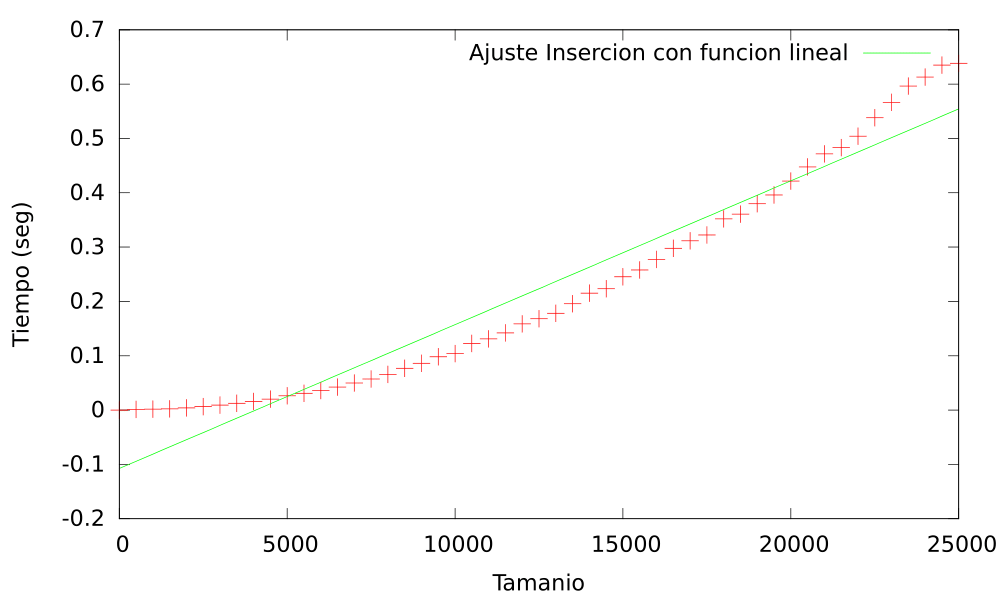
\includegraphics[totalheight=8cm]{img/ajusteInsercion_lineal}
		\caption{Ajuste Inserción con función lineal}
		\label{fig:ajusteInsercion_lineal}
	\end{figure}
	
	\begin{figure}[h]
		\centering
		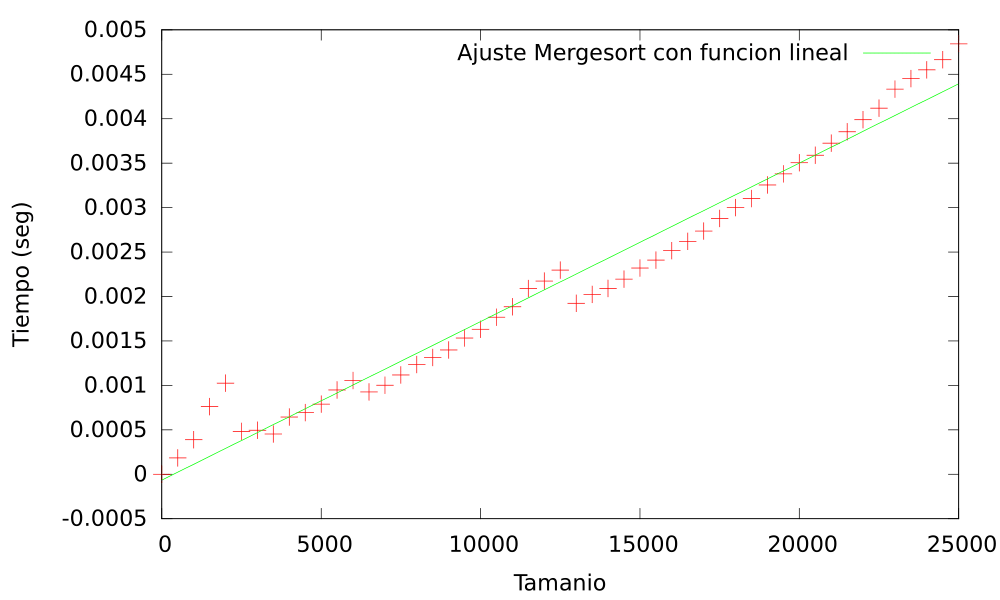
\includegraphics[totalheight=8cm]{img/ajusteMergesort_lineal}
		\caption{Ajuste Mergesort con función lineal}
		\label{fig:ajusteMergesort_lineal}
	\end{figure}
	
	\section{Comparacion tiempos distintos computadores}
	
	\begin{figure}[h]
		\centering
		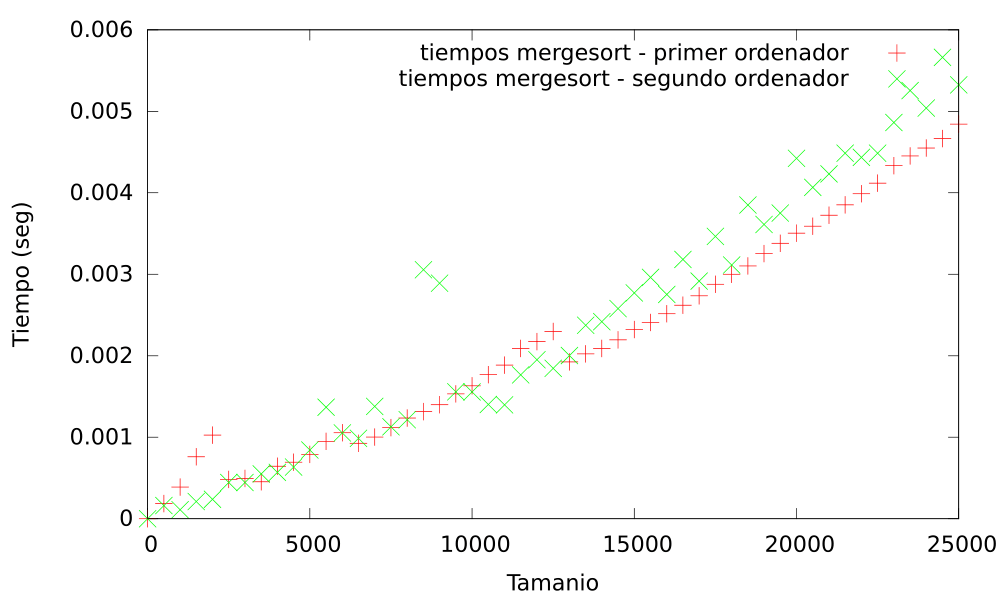
\includegraphics[totalheight=8cm]{img/compMergesort}
		\caption{Comparación Mergesort entre distintos computadores}
		\label{fig:compMergesort}
	\end{figure}
	
	\begin{figure}[h]
		\centering
		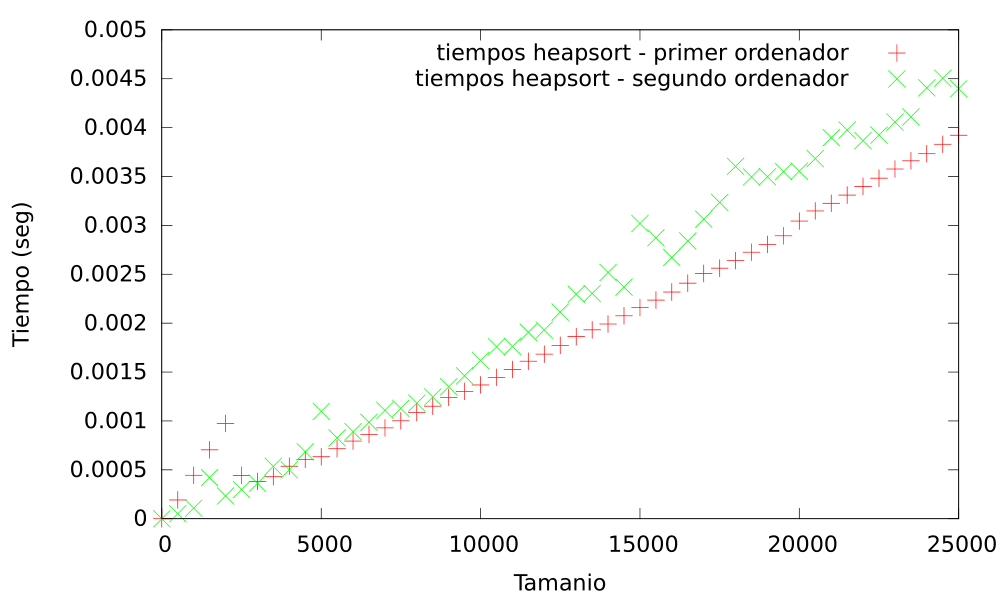
\includegraphics[totalheight=8cm]{img/compHeapsort}
		\caption{Comparación Heapsort entre distintos computadores}
		\label{fig:compHeapsort}
	\end{figure}
	
	\begin{figure}[h]
		\centering
		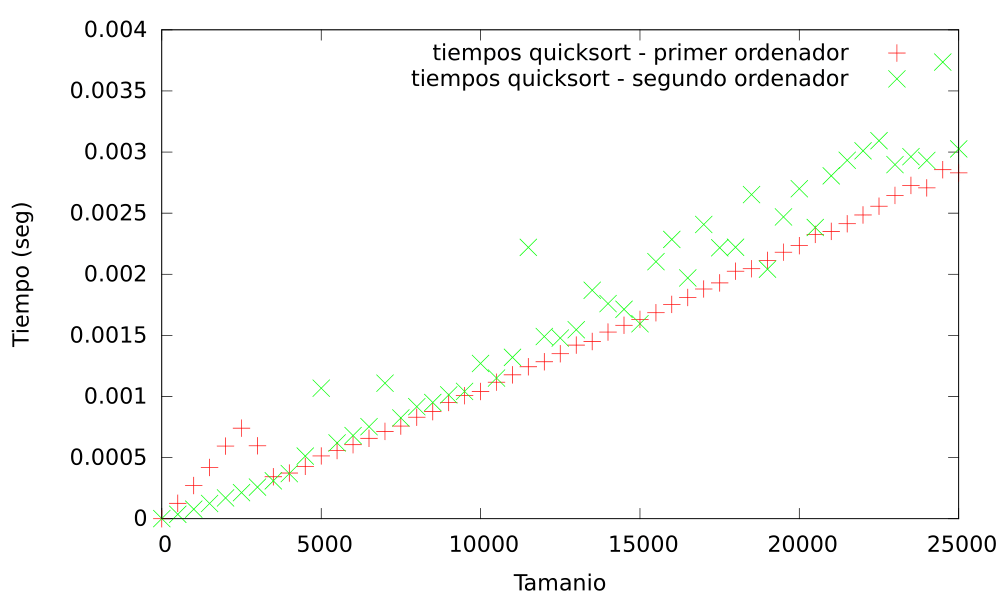
\includegraphics[totalheight=8cm]{img/compQuicksort}
		\caption{Comparación Quicksort entre distintos computadores}
		\label{fig:compQuicksort}
	\end{figure}
	
	\begin{figure}[h]
		\centering
		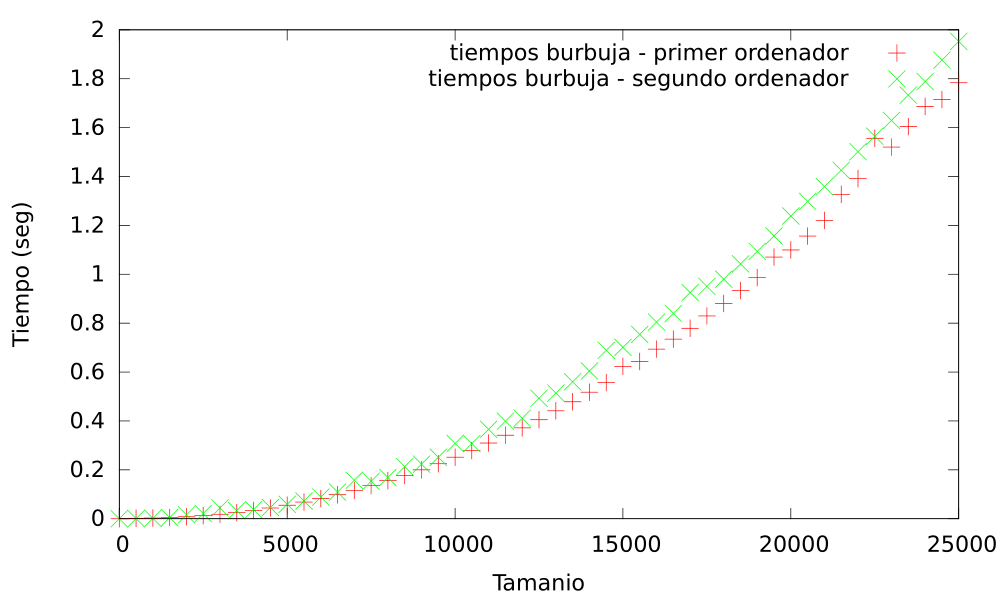
\includegraphics[totalheight=8cm]{img/compBurbuja}
		\caption{Comparación Burbuja entre distintos computadores}
		\label{fig:compBurbuja}
	\end{figure}
	
	\begin{figure}[h]
		\centering
		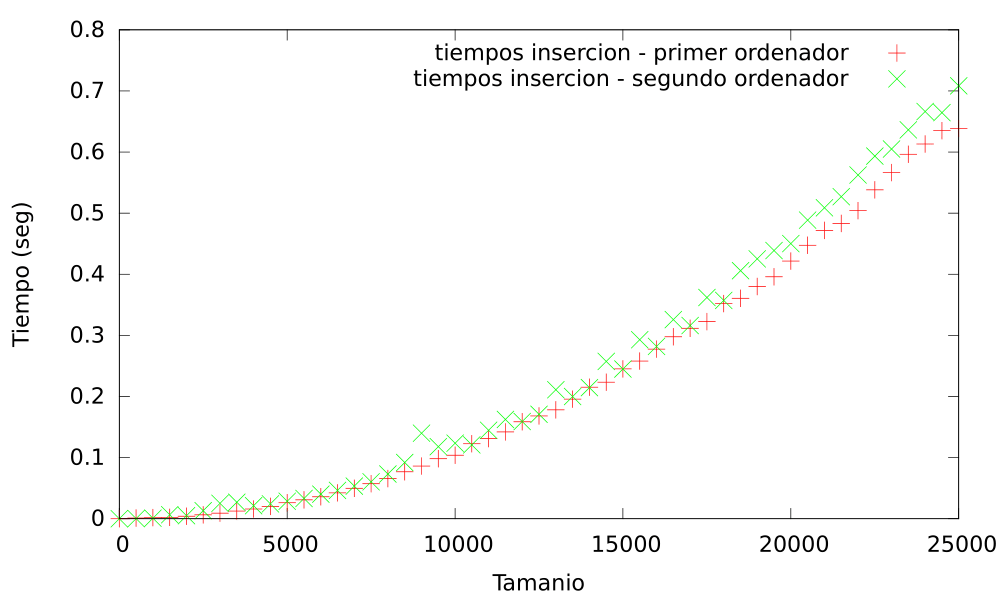
\includegraphics[totalheight=8cm]{img/compInsercion}
		\caption{Comparación Inserción entre distintos computadores}
		\label{fig:compInsercion}
	\end{figure}
	
	\begin{figure}[h]
		\centering
		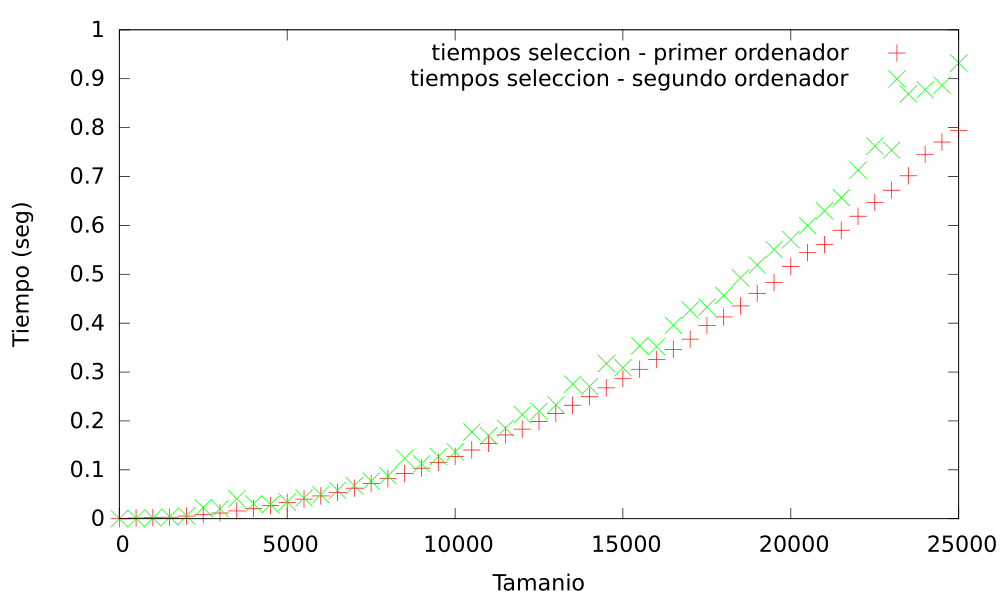
\includegraphics[totalheight=8cm]{img/compSeleccion}
		\caption{Comparación Selección entre distintos computadores}
		\label{fig:compSeleccion}
	\end{figure}
	
	\begin{figure}[h]
		\centering
		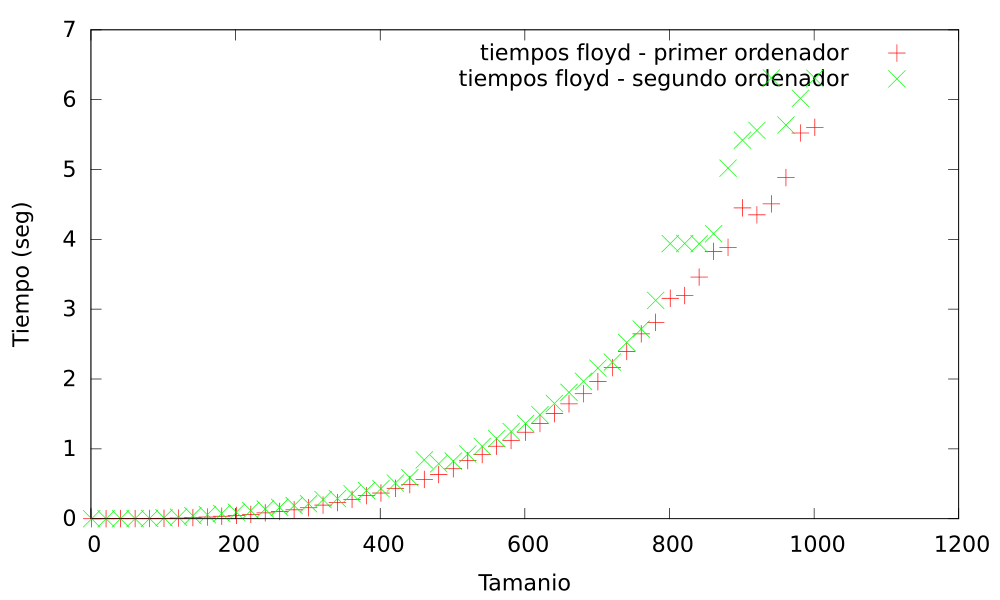
\includegraphics[totalheight=8cm]{img/compFloyd}
		\caption{Comparación Floyd entre distintos computadores}
		\label{fig:compFloyd}
	\end{figure}
	
	\begin{figure}[h]
		\centering
		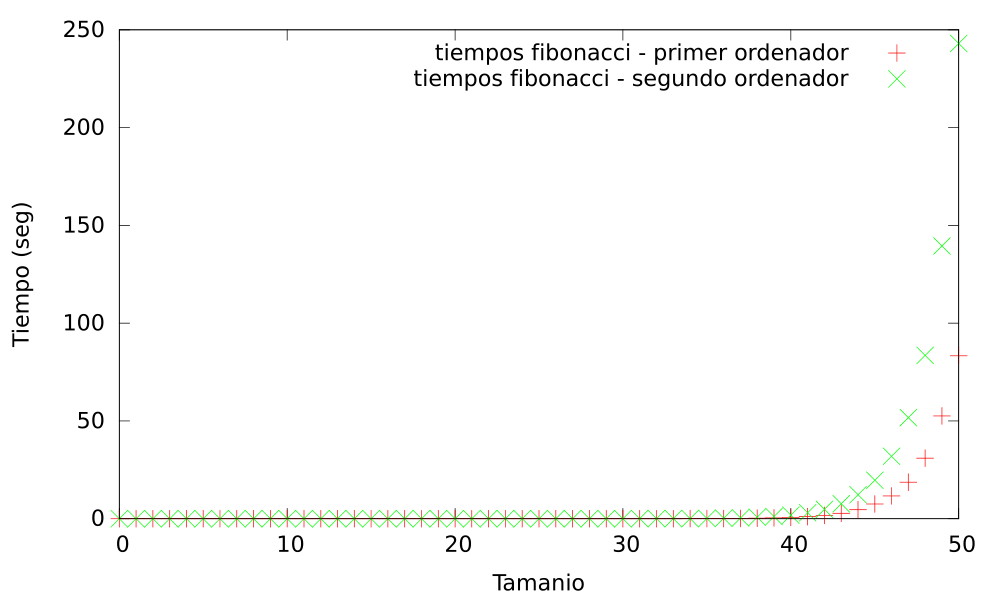
\includegraphics[totalheight=8cm]{img/compFibonacci}
		\caption{Comparación Fibonacci entre distintos computadores}
		\label{fig:compFibonacci}
	\end{figure}
	
\end{document}
